\xchapter{Ciclo de vida de software acadêmico de análise estática}{}
\label{estudo3}

Este capítulo apresenta
um estudo para caracterização de software acadêmico de análise estática,
em relação ao estágio de evolução no modelo {\it ``Staged Model for Software Evolution''},
em termos de número de lançamentos e
tamanho em número de módulos no código fonte.

O estudo avaliou o ciclo de vida de software acadêmico coletando
dados do código fonte através de análise estática com o apoio da
ferramenta Analizo, esta análise revelou que a maior parte dos projetos
estão em estágio inicial de desenvolvimento ou encerrados.

A seção \ref{estudo3:introducao} contextualiza o estudo,
a seção \ref{estudo3:escopo} descreve o objetivo e apresenta as questões de pesquisa,
a seção \ref{estudo3:planejamento} apresenta um planejamento do estudo,
as seções \ref{estudo3:preparacao} e \ref{estudo3:coleta} apresentam detalhes sobre a preparação e execução da coleta de dados,
as seções \ref{estudo3:analise} e \ref{estudo3:interpretacao} apresentam a análise e interpretação dos dados e
a seção \ref{estudo3:conclusoes} traça as conclusões finais deste estudo.

\section{Motivação} \label{estudo3:introducao} % {{{

%Neste estudo caracterizamos projetos de software acadêmico de análise
%estática quanto ao seu estágio no ciclo de vida de software de acordo o modelo
%{\it ``Staged Model for Software Evolution''}
%, neste modelo

O ciclo de vida de um produto de software tem início no estágio
de evolução chamado {\it ``Initial development''}, onde a primeira versão funcional
do software é desenvolvida, passando pelas fases {\it
``Evolution''}, {\it ``Servicing''}, {\it ``Phaseout''}, e encerrando seu ciclo
na fase {\it ``Closedown''}, quando as empresas dedentoras do
software o retiram do mercado \cite{rajlich2000staged}.

Em modelos de produção distintos e não-tradicionais, como é o modelo de
software acadêmico ou software livre, por exemplo, este ciclo de vida pode
variar. No modelo {\it ``Staged Model for Software Evolution''} adaptado a
projetos software livre \cite{capiluppi2007adapting}, por exemplo, o ciclo de
vida não se encerra na fase de {\it ``Closedown''}, uma vez que estes projetos
não são retirados do mercado por empresas, podendo haver um caminho de retorno
entre as diversas fases, incluindo o retorno para a fase {\it
``Initial development''}, por exemplo.

Os projetos de software acadêmico caracterizados neste estudo são considerados
como projetos de software livre sob a perspectiva do modelo proposto por
\citeonline{capiluppi2007adapting}, uma vez que não há entre eles projetos
comerciais de propriedade exclusiva de empresas, enquadram-se muito melhor
neste modelo do que no modelo tradicional de software comercial não-livre
originalmente proposto por \citeonline{rajlich2000staged}.

A caracterização dos projetos de software acadêmico de análise estática quando
ao ciclo de vida será feito sob a perspectiva de cientistas desenvolvedores e
usuários finais de software interessados em compreender em que estágio de
desenovolvimento e evolução estão os projetos do ecossistema de software
acadêmico de análise estática uma vez que saber em que fase um software está é
útil ao se tomar decisão de adotar um certo software como uso ou mesmo como
objeto de contribuição.

Neste estudo, módulo refere-se as partes que compõe um sistema de software.  A
maioria dos paradigmas de desenvolvimento de software possui uma ou mais
construções que fazem o papel de módulo -- ``classes'', ``aspectos'', ``tipos
abstratos de dados'', ou ``arquivos-fonte'' -- para as quais serão calculadas
para cada projeto.

% }}}

\section{Escopo} \label{estudo3:escopo} % {{{

Projetos de software acadêmico de análise estática publicados nas 
conferências ASE e SCAM 
são nosso principal objeto de estudo.
Queremos saber em qual estágio de evolução estão os projetos de software
acadêmico de análise estática publicados nas conferências ASE e SCAM.

O objetivo da pesquisa está definido segundo a estrutura GQM \cite{van1999goal}.

\subsection{Definição do Objetivo}

\begin{description}

  \item{\bf Objeto de estudo.}
    O objeto de estudo são projetos de software acadêmico de análise estática
    publicados em artigos científicos e seu estágio de evolução no ciclo de
    vida de software, conforme definido na seção~\ref{estudo3:introducao}.

  \item{\bf Propósito.}
    O propósito do estudo é caracterizar em qual estágio de evolução
    encontra-se cada software acadêmico de análise estática. O estudo
    contribuirá para a análise da desordem disfuncional caótica no domínio de
    análise estática. 

  \item{\bf Perspectiva.}
    A perspectiva considerada é a do cientista desenvolvedor e usuário final, isto é, o pesquisador
    que deseja saber em que estágio de evolução estão os projetos de software acadêmico do domínio
    de interesse. A perspectiva a ser considerada é a do pesquisador que deseja
    conhecer ferramentas de análise estática para uso em sua pesquisa.

  \item{\bf Foco de qualidade.}
    O principal foco de qualidade estudado é ciclo de vida do software
    acadêmico de análise estática, com ênfase nos aspectos de lançamentos e
    versões do projeto, especialmente sobre o tamanho do software em número de
    módulos.

  \item{\bf Contexto.}
    O estudo foi conduzido com projetos de software acadêmico de análise
    estática publicados nas conferências ASE e SCAM.

\end{description}

\subsection{Sumário da Definição}

Analisar os \textit{projetos de software acadêmico de análise estática} publicados
com o propósito de \textit{caracterizá-los}
com respeito ao seu \textit{ciclo de vida}
na perspectiva de \textit{cientistas usuários finais e desenvolvedores de software}
no contexto das \textit{conferências de Engenharia de Software ASE e SCAM}.

\subsection{Questões de Pesquisa}

Neste estudo as seguintes questões de pesquisa, a respeito dos projetos de
software acadêmico de análise estática publicados nas conferências ASE e SCAM,
e seu ciclo de vida serão investigadas:

\newcommand{\EstudoTresQuestaoUm}{
  Em qual estágio de evolução estão os projetos de software acadêmico de
  análise estática publicados nas conferências ASE e SCAM em relação ao seu
  ciclo de vida?
}

\begin{description}
  \item [Q1:] \EstudoTresQuestaoUm
\end{description}

\subsection{Métricas}

Para responder às questões de pesquisas, as seguintes métricas serão usadas:

\begin{enumerate}
  \item Número de lançamentos de cada projeto com informações sobre versão e data
  \item Número de lançamentos com código fonte disponível para download
  \item Número de módulos no código fonte de cada lançamento/versão
%  \item Número contribuidores no repositório de código fonte dos projetos de software acadêmico de análise estática.
\end{enumerate}

% }}}

\section{Planejamento do Estudo} \label{estudo3:planejamento} % {{{

Este estudo foi realizado a partir de uma análise inicial dos dados existentes
de cada software, coletados previamente nos Capítulos \ref{estudo1} e
\ref{estudo2}, a partir dessa análise define-se quais projetos são candidatos a
terem mais dados coletados para compor a caracterização do seu ciclo de vida. Ao
final do estudo cada projeto será caracterizado em um dos estágios
de evolução apresentados na seção \ref{estudo3:introducao}.

Nesta análise inicial deve-se identificar entre os projetos de software
acadêmico quais possuem disponibilidade de download, ou ao menos, presença
oficial online com informações do projeto sobre lançamentos, onde as seguintes
informações serão coletadas:

\begin{itemize}
  \item Número da versão
  \item Data do lançamento
  \item URL para download do código fonte
\end{itemize}

A fonte para coleta desses dados são o site do projeto, manuais, código fonte e
repositórios, usualmente será utilizado mais de uma fonte para compor todas as
informações sobre os lançamentos de um certo software. Não é raro que os
projetos mudem a forma de lançamento, passando de um formato para outro, de uma
plataforma a outra, entre outras mudanças, essas informações devem ser
investigadas a fim de encontrar o máximo de informação possível.

%As informações sobre lançamentos foram coletadas manualmente em arquivos de
%changelog, no site do projeto, ou em tags no próprio repositório de código
%fonter. O número de commits foi coletado com o uso do git via linha de comando,
%o cálculo e coleta da métrica de complexidade estrutural do código fonte foi
%coletada com software de análise estática Analizo.

Os projetos sem presença oficial online ou sem disponibilidade de download, ou
seja, com a URL indicada pelos seus autores originais indisponível,
não terão, consequentemente, informações sobre os lançamentos, dessa forma, estes
projetos serão caracterizados como software com ciclo de vida encerrado ({\it
Closedown}), uma vez que eles estão indisponíveis e inacessíveis a qualquer
potencial usuário interessado em utilizar o software.

%{\it ``Staged Model for Software Evolution''}, estes projetos serão
%caracterizados como estando na fase {\it ``Closedown''}.

Os demais projetos, aqueles com presença online, e com código fonte disponível,
tiveram o código fonte de cada lançamento copiado localmente para análise
estática e coleta da métrica representando o tamanho do software em número de
módulos, foi feito o download do código fonte de cada versão e a ferramenta de
análise estática Analizo foi utilizada para extrair as informações do código
fonte.

Analizo é software livre, distribuído sob a licença GNU General Public License
versão 3. Seu código-fonte, bem como pacotes binários, manuais e tutoriais
podem ser obtidos em \url{http://www.analizo.org}. Analizo é escrito em Perl,
sua última versão 1.19.1 lançada em 01 de Setembro de 2016 foi a versão
utilizada neste estudo.

Apenas os projetos escritos nas linguagens suportadas pelo Analizo foram
analisados, apenas C, C++ C\# e Java. O código fonte dos projetos escritos em
outras linguagens de programação não serão analisados, estes projetos serão caracterizados
com base nas outras informações disponíveis ou serão definidos como {\it Desconhecido} quando não for possível determinar o estágio de evolução com as informações disponíveis. Projetos com apenas um
lançamento serão considerados projetos em estágio inicial de desenvolvimento
({\it Initial development}).

%não é possível determinar outras fases
%olhando apenas os dados coletados aqui, mesmo que sejam projetos com
%código fonte disponível, a métrica indicando o tamanho em número de módulos
%foi coletada para se ter uma dimensão do tamanho de cada projeto, mas
%será caracterizado automaticamente como 

%caracterizados em relação ao estágio de
%evolução no ciclo de vida.

%Em seguida entre os demais projetos, selecionamos os projetos com
%disponibilidade de código fonte para uma análise evolutiva entre os
%lançamentos, para cada lançamento será obtido o código fonte e será extraído
%métricas representando o número de módulos para avaliação histórica.

%Analisar historicamente (evolucao) dos projetos com maior número de releases
%(com codigo dessas releases) e que já tenha coletado as metricas (ja coletei
%varias versoes de alguns projetos), a analise individual.


%poucos releases, digamos, abaixo de 5, não serão analisados em
%detalhes na avaliação histórica, mas terão os dados das métricas analisados
%para definir o estágio de evolução.

%Os projetos sem disponibilidade de
%download não serão caracterizados quanto ao seu ciclo de vida uma vez que os
%indícios para realizar este estudo está centrado na disponibilidade de código
%fonte.

% }}}

\section{Preparação} \label{estudo3:preparacao} % {{{

Seguindo o planejamento apresentado na seção \ref{estudo3:planejamento},
preparamos os arquivos e templates necessários para realizar a coleta e análise
dos dados, o conjunto de projetos de software acadêmico de análise estática e
os dados coletados nos Capítulos \ref{estudo1} e \ref{estudo2} serão também
utilizados aqui neste estudo.

Para cada projeto foi criado um arquivo \texttt{releases.yml} com a estrutura
apresentada na Listagem \ref{releases-yml}, nele serão registradas as
informações sobre os lançamentos de cada software. Os arquivos foram criados
manualmente, para os projetos sem informações sobre lançamentos o arquivo será
criado com um único campo indicando indisponibilidade com o seguinte conteúdo
\texttt{source: unavailable}.

\begin{lstlisting}[
caption={Arquivo releases.yml.},
label={releases-yml},
frame=single,
numbers=left
]
  source:
  versions:
    - version:
      source:
      released_at:
    - version:
      source:
      released_at:
\end{lstlisting}

Após criar os arquivos para a coleta de informações sobre os lançamentos,
implementamos um arquivo de template em
\texttt{templates/releases-table.tex.epl} para agregar os dados e apresentá-los
na seção \ref{estudo3:coleta}, Tabela \ref{releases-table}.

%apresentados, o arquivo de template criado está em
%, este arquivo gera o
%\texttt{documents/releases-table.tex} 

O Analizo e suas dependências foram instaladas, um script para automatizar a
execução da ferramenta {\it analizo metrics} para coletar o número de módulos
de cada lançamento foi desenvolvido. Este script, disponível em
\texttt{bin/run-analizo}, foi implementado em linguagem Perl e será apresentado
em mais detalhes no Apêndice \ref{reproducibilidade-do-estudo}.

%, definimos uma estrutura de diretórios e localização dos arquivos, etc.  

As métricas serão agregadas no arquivo CSV \texttt{documents/metrics.csv}
gerado pelo template \texttt{templates/metrics.csv.epl}, este template consulta
os arquivos com os dados de cada lançamento criado pela execução do {\it analizo metrics}
e exibe, para cada projeto, todos os lançamentos e suas métricas.

Por fim, definimos uma estrutura para adicionar aos arquivos \texttt{software.yml} de
cada projeto a informação final sobre o atual estágio de evolução em relação ao
ciclo de vida do software, conforme mostra a Listagem \ref{software-yml-life-cycle}.

\begin{lstlisting}[
caption={Campos adicionados ao arquivo software.yml de cada projeto.},
label={software-yml-life-cycle},
frame=single,
numbers=left
]
  life_cycle:
    stage:
    review:
\end{lstlisting}

O campo \texttt{review} foi utilizado para registrar anotações em forma livre
sobre a análise dos dados, a avaliação de cada projeto é realizada
inspecionando manualmente os dados coletados, incluindo dados trazidos pelos
estudos anteriores, o campo \texttt{stage} contém o resultado final da
caracterização do ciclo de vida de cada software, este campo assumirá um dos
estágios de evolução conforme o modelo de evolução apresentado em
\ref{estudo3:introducao}.

%Analisar apenas os projetos com código fonte suportado pelo Analizo (C, C++ e Java),
%Derailer é Ruby, Flowgen é Python, PHP AiR é Rascal, protopurity é Javascript,
%Pseudogen é Python, TEBA é Perl, Wrangler é Erlang,
%o e-munity e mygcc são basicamente o código do GCC, n faz sentido coletar métricas para ele.

%Para os outros projetos, com código fonte disponível, copiamos localmente o código fonte
%e executamos o analizo metrics para coletar a métrica de complexidade estrutural, tamanho em
%linhas de código e número de classes.

% }}}

\section{Coleta de Dados} \label{estudo3:coleta} % {{{

Seguindo o planejamento e preparação descritos nas seções
\ref{estudo3:planejamento} e \ref{estudo3:preparacao}, iniciamos a coleta dos
dados, incluindo a coleta do número de lançamentos de cada projeto, informações
e código fonte de cada lançamento, bem como a métrica representando o número de
módulos do software em cada versão. Coletamos os dados sobre lançamentos,
fizemos o download do código fonte e executamos a ferramenta \texttt{analizo
metrics} para cada projeto, em cada versão.

Foi encontrado ao todo \ReleasesCount \ lançamentos, coletamos para cada
lançamento, quando disponível, número da versão, data de lançamento e URL para
download do código fonte. Destes lançamentos, \ReleasesAvailableCount \ possui
informação para download, 5 destes releases não tem código fonte, apenas
binários do software \texttt{s33}. Assim, deste total extraímos métricas
de código fonte de \ReleasesMetricsCount \ lançamentos.

Este total de métricas foi extraído de um conjunto de \ProjectsAnalizedCount \
projetos, os demais projetos não possuem código fonte disponível ou são
escritos em linguagem de programação não suportada pelo Analizo. Entre os anos
de \ReleasesYearFirst \ e \ReleasesYearLast.

%a data do lançamento, o endereço para download
%do código fonte da versão, e número da versão, fazer download de cada versão
%em código fonte, apenas entre os suportados pelo Analizo para coleta de métricas.

%Os dados coletados incluem a caracterização das ferramentas de análise
%estática, bem como, os valores das métricas de código-fonte de complexidade
%estrutural para cada ferramenta.

%Os projetos com poucas releases, sem informação sobre datas de lançamentos,
%serão considerados em estágio inicial de desenvolvimento. Para coletar as
%versões e datas dos projetos que não disponibilizam no site olhamos o código
%fonte quando disponível em arquivos NEWS, ChangeLog, etc.

%criamos as entradas abaixono arquivo software.yml, e nele anotamos
%a avaliacao sobre o ciclo de vida e no campo stage definimos o estágio
%de cada projeto

%life_cycle:
%  stage: Initial development
%  review: 1 versão sem data, 1 contribuicao em 2011 outra 2013, 1 uso em 2017

Os lançamentos coletados do repositório, código fonte, sites, devem ser
organizados em ordem de data de lançamento, os mais antigos primeiros, numa
lista em ordem, sendo o último release o lançamento mais recente. Isto é
necessário uma vez que o número de versão de cada projeto não segue o mesmo
padrão, alterando de formatos entre releases distintos, a data de lançamento de
cada release também nem sempre está disponível, então a coleta deve garantir
que haja alguma ordem, então no momento da coleta deve-se avaliar a ordem dos
lançamentos e registrar no arquivo \texttt{releases.yml} na ordem correta.

% }}}

\section{Análise dos Dados} \label{estudo3:analise} % {{{

Analisamos as métricas e a variação em número de módulos entre as versões dos
projetos com lançamentos e código fonte disponível, analisamos também as
menções do tipo Uso e Contribuiçao para determinar se há atividade recente para
os projetos sem lançamentos atuais.

Iremos considerar projetos em fase de serviço ({it Servicing}) aqueles que
apresentem variação pequena entre os lançamentos em relação ao tamanho do
projeto, em termos de número de módulos, abaixo de 10\% de variação ao longo
das versões será considerado {\it Servicing}, acima de 10\% está em evolução
({\it Evolution}), este número 10\% foi emprestado do trabalho de
\citeonline{capiluppi2007adapting}.
%estudo pegamos esse numero da secao 3.3.1 do staged model adaptado a floss.

%para definir entre os que não tem atualização a mais de 5 anos, verificar as
%menções, se houver menções com uso/contribuição é possível que esteja em serving,
%caso contrário está em phase-out

%A ... apresenta em conjunto o número de releases total
%de cada projeto em relação ao número total de menções encontradas nas bases ACM e IEEE,
%os projetos sem informação de releases foi excluído do gráfico.

Cinco projetos não puderam ser caracterizados em relação ao estágio de
evolução, a Tabela \ref{releases-table} apreseta a caracterização final de
todos os projetos incluindo o número total de lançamentos e o período em que
estes lançamentos aconteceram.

\begin{longtable}{ l c c l | l c c l }
\caption{Número e período dos lançamentos de software acadêmico de análise estática.}
\label{releases-table} \\
  \hline
  \hhline{ l c c l | l c c l |}
  \endfirsthead
  \hhline{ l c c l | l c c l |}
  \hline
  \multirow{2}{*}{\textbf{ID}} & \multicolumn{2}{c}{\textbf{Lançamentos}} & \multirow{2}{*}{\textbf{Evolução}} & \multirow{2}{*}{\textbf{ID}} & \multicolumn{2}{c}{\textbf{Lançamentos}} & \multirow{2}{*}{\textbf{Evolução}} \\
           & \textbf{\#} & \textbf{Período} &                &            & \textbf{\#} & \textbf{Período} &  \\
  \hline
  \hhline{ l c c l | l c c l |}
  \endhead
  \hhline{----|----}
  \multicolumn{8}{c}{continua na próxima página} \\
  \hhline{----|----} \endfoot
  \hhline{----|----} \endlastfoot
  \multirow{2}{*}{\textbf{ID}} & \multicolumn{2}{c}{\textbf{Lançamentos}} & \multirow{2}{*}{\textbf{Evolução}} & \multirow{2}{*}{\textbf{ID}} & \multicolumn{2}{c}{\textbf{Lançamentos}} & \multirow{2}{*}{\textbf{Evolução}} \\
           & \textbf{\#} & \textbf{Período} &                &            & \textbf{\#} & \textbf{Período} &  \\
  \hline
      \texttt{s1} & 7 & 2015-2017 & Evolution &
        \texttt{s31} & - & - & Closedown  \\
      \texttt{s2} & 4 & 2010-2012 & Initial development &
        \texttt{s32} & 1 & 2006 & Desconhecido  \\
      \texttt{s3} & - & - & Closedown &
        \texttt{s33} & 5 & 2007-2010 & Desconhecido  \\
      \texttt{s4} & - & - & Closedown &
        \texttt{s34} & 1 & 2017 & Initial development  \\
      \texttt{s5} & - & - & Closedown &
        \texttt{s35} & 1 & 2017 & Initial development  \\
      \texttt{s6} & 36 & 2013-2017 & Servicing &
        \texttt{s36} & - & - & Closedown  \\
      \texttt{s7} & 7 & 2001-2004 & Initial development &
        \texttt{s37} & 5 & - & Initial development  \\
      \texttt{s8} & 4 & 2005 & Initial development &
        \texttt{s38} & - & - & Closedown  \\
      \texttt{s9} & - & - & Closedown &
        \texttt{s39} & - & - & Closedown  \\
      \texttt{s10} & 4 & - & Initial development &
        \texttt{s40} & 4 & 2011-2014 & Desconhecido  \\
      \texttt{s11} & - & - & Closedown &
        \texttt{s41} & - & - & Phaseout  \\
      \texttt{s12} & 2 & 2013-2014 & Initial development &
        \texttt{s42} & 1 & 2017 & Initial development  \\
      \texttt{s13} & - & - & Closedown &
        \texttt{s43} & 1 & 2008 & Initial development  \\
      \texttt{s14} & 1 & 2014 & Initial development &
        \texttt{s44} & - & - & Closedown  \\
      \texttt{s15} & - & - & Closedown &
        \texttt{s45} & - & - & Closedown  \\
      \texttt{s17} & 1 & 2014 & Initial development &
        \texttt{s46} & 5 & 2009-2010 & Initial development  \\
      \texttt{s16} & 1 & - & Initial development &
        \texttt{s47} & - & - & Closedown  \\
      \texttt{s18} & 25 & 2015-2017 & Servicing &
        \texttt{s48} & - & - & Closedown  \\
      \texttt{s19} & - & - & Closedown &
        \texttt{s49} & - & - & Closedown  \\
      \texttt{s20} & - & - & Closedown &
        \texttt{s50} & 6 & 2015-2017 & Evolution  \\
      \texttt{s21} & 1 & - & Initial development &
        \texttt{s51} & 18 & 2012-2016 & Servicing  \\
      \texttt{s22} & 1 & 2017 & Initial development &
        \texttt{s52} & 14 & 2011-2015 & Initial development  \\
      \texttt{s23} & - & - & Closedown &
        \texttt{s53} & - & - & Closedown  \\
      \texttt{s24} & 1 & - & Closedown &
        \texttt{s54} & 1 & - & Closedown  \\
      \texttt{s25} & 3 & 2013-2015 & Initial development &
        \texttt{s55} & 21 & 2010-2016 & Desconhecido  \\
      \texttt{s26} & 22 & 2013-2017 & Servicing &
        \texttt{s56} & - & - & Closedown  \\
      \texttt{s27} & 1 & - & Initial development &
        \texttt{s57} & - & - & Closedown  \\
      \texttt{s28} & 26 & 2013-2017 & Servicing &
        \texttt{s58} & 37 & 2006-2017 & Servicing  \\
      \texttt{s29} & 1 & 2013 & Initial development &
        \texttt{s59} & 34 & 2013-2015 & Desconhecido  \\
      \texttt{s30} & - & - & Closedown &
        \texttt{s60} & - & - & Closedown  \\
\end{longtable}


O projeto s59 não foi caracterizado por possuir muitas versões entre 2013 e
2015 mas por escrito em Erlang não foi possível analisar o código fonte para
determinar em qual fase se encontra, s55 também possui muitos lançamentos entre
2010 e 2016 mas apesar disso está escrito em Perl, s40 aapesar de poucos
lançamentos, apenas 4, a falta de dados sobre código fonte pois está escrito em
Rascal ..., s33 apesar de poucas versões olhar o código é necessário para ter
idéia de como o código mudou mas só tem disponível binários, s32 projeto com
histórico entre 2004 e 2006 mas com a distribuição de código fonte bastante
confusa dificultando compreender quais pacotes fazem parte de qual versão ou
lançamento.

% }}}

\section{Interpretação dos Resultados} \label{estudo3:interpretacao} % {{{

\subsection{Q1 - \EstudoTresQuestaoUm}

Os \SoftwareCount \ projetos de software acadêmico de análise estática estão em
sua maioria em estágio inicial de desenvolvimento ou encerrados, representando
76\% de todos os projetos. Os demais 24\% dos projetos estão distribuídos entre
projetos em evolução, serviço, encerrando ou não puderam ser determinados,
conforme Figura \ref{life-cycle}.

\begin{figure}[h]
  \begin{minipage}{0.5\textwidth}
    \centering
    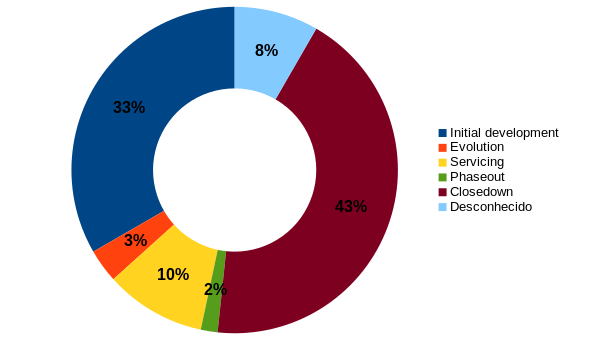
\includegraphics[scale=0.55]{imagens/life-cycle-pie.png}
  \end{minipage}
  \begin{minipage}{0.5\textwidth}
    \centering
    \begin{tabular}{l c}
  \hline
  {\bf Estágio} & {\bf Projetos} \\
  \hline
    Initial development & 20 \\
    Evolution & 2 \\
    Servicing & 6 \\
    Phaseout & 3 \\
    Closedown & 24 \\
    Desconhecido & 5 \\
  \hline
\end{tabular}

  \end{minipage}
  \caption{Número total de projetos identificados em cada estágio de evolução.}
  \label{life-cycle}
\end{figure}

Entre os projetos em fase de evolução ou serviço estão aqueles com maior número
de lançamentos.

\begin{figure}[h]
  \begin{minipage}{0.32\textwidth}
    \centering
    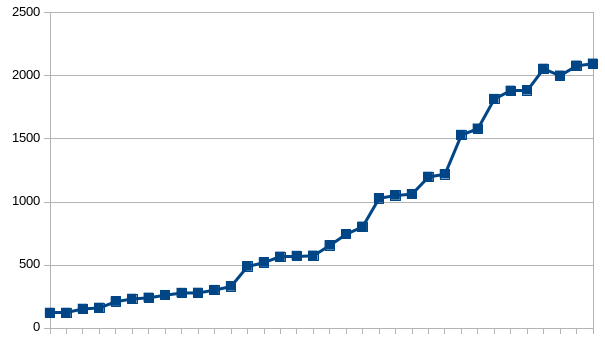
\includegraphics[scale=0.32]{imagens/evolution-s6.png}
    \texttt{s6}
  \end{minipage}
  \begin{minipage}{0.32\textwidth}
    \centering
    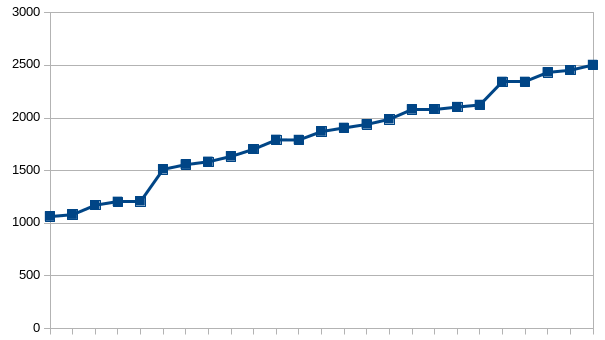
\includegraphics[scale=0.32]{imagens/evolution-s18.png}
    \texttt{s18}
  \end{minipage}
  \begin{minipage}{0.32\textwidth}
    \centering
    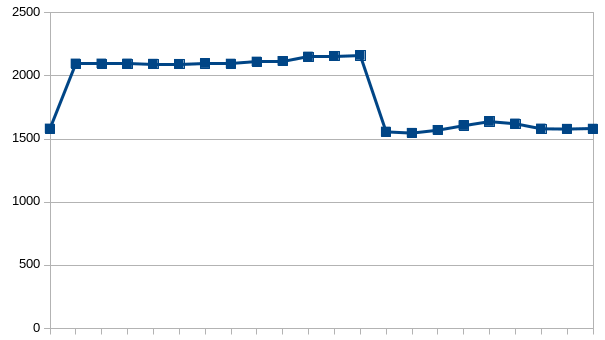
\includegraphics[scale=0.32]{imagens/evolution-s26.png}
    \texttt{s26}
  \end{minipage}

\vspace{3mm}

  \begin{minipage}{0.32\textwidth}
    \centering
    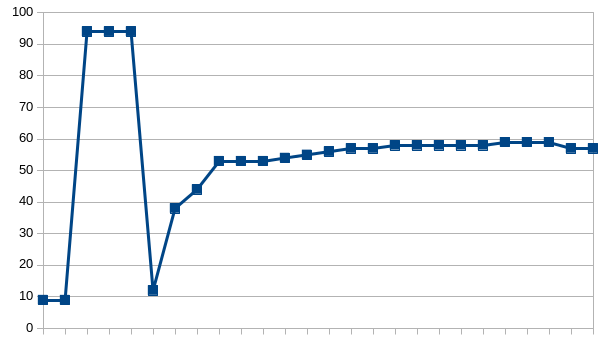
\includegraphics[scale=0.32]{imagens/evolution-s28.png}
    \texttt{s28}
  \end{minipage}
  \begin{minipage}{0.32\textwidth}
    \centering
    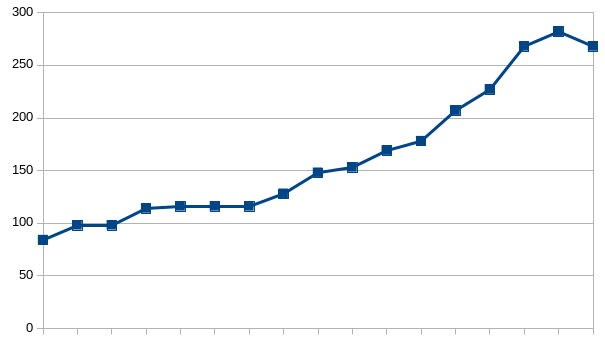
\includegraphics[scale=0.32]{imagens/evolution-s51.png}
    \texttt{s51}
  \end{minipage}
  \begin{minipage}{0.32\textwidth}
    \centering
    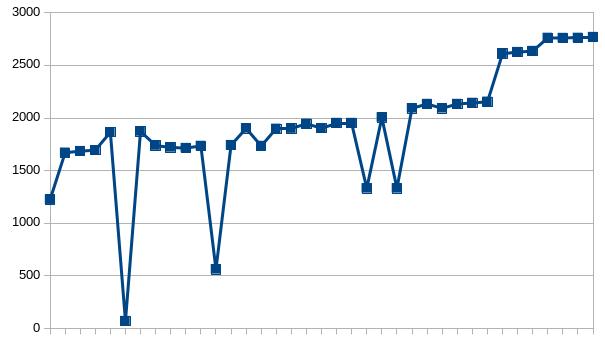
\includegraphics[scale=0.32]{imagens/evolution-s58.png}
    \texttt{s58}
  \end{minipage}
  \caption{Variação no número de módulos dos projetos em fase de {\it Servicing}.}
  \label{evolution-graph}
\end{figure}

% }}}

\section{Ameaças à validade} % {{{

Toda a análise e interpretação dos resultados tomou como base apenas os dados
coletados do site, publicações, e repositórios dos projetos de software
acadêmico de análise estática, o fato de não incluirmos coleta de dados a
partir das pessoas envolvidas nos projetos pode enfraquecer alguma conclusão no
sentido de que alguns projetos podem ter definições explícitas por parte dos
seus desenvolvedores mas que não se refletem ainda nos documentos dos projetos,
apesar disso o nosso estudo tem um caráter exploratório, com interesse especial em
uma figura geral do domínio de análise estática e não necessariamente trazer
evidências sobre os projetos inidivualmente.

% }}}

\section{Conclusões} \label{estudo3:conclusoes} % {{{

Este estudo coletou informações de \ReleasesCount \ lançamentos em relação a
\ProjectsWithReleasesCount \ projetos de software acadêmico de análise
estática. Analisou e extraiu o número de módulos do código fonte de
\ReleasesMetricsCount \ versões distintas destes projetos.

A partir destes dados caracterizou cada um dos \SoftwareCount \ projetos
estudados em relação ao estágio de evolução do ciclo de vida do software e
identificou que a grande maioria encontra-se em estado inicial de
desenvolvimento ou encerrados (76\%).

Apenas 2 projetos encontram-se em evoluçao atualmente, com variação no número
de módulos nos últimos lançamentos recentes superior a 10\%. E 6 projetos em
fase de serviço, indicando que são projetos estáveis com atualizações
constantes mas com pouca variação na base de código do projeto.

Os dados, interpretações e conclusões deste estudo e dos dois estudos
anteriores apresentados nos Capítulos \ref{estudo1} e \ref{estudo2} serão
analisados em conjunto e discutidos no Capítulo seguinte sob uma mesma
perspectiva em relaçao a sustentabilidade técnica do ecossistema de software
acadêmico de análise estática, no recorte de projetos selecionados nas
conferências de Engenharia de Software ASE e SCAM, entre menções encontradas
nas bases ACM e IEEE, e com análise ao nível de código fonte dos projetos
escritos em C, C++ e Java.

% }}}

%% O percentil 75 tem muitos valores zero, os percentis 90 e 95 sao pracitamente iguais 
%% na comparacao, os maiores sao geralmente tb maior no outro, exceto uns 2 exemplos:
%% smatch-0.3/EJB e pmd-src-5.3.7/wap-2.1.

%Os valores encontrados serão avaliados sempre tendo em vista os intervalos
%sugeridos na Tabela \ref{valores-frequentes}, esta tabela traz os valores encontrados
%no estudo que estamos replicando em parte \cite{Meirelles2013}.

%\begin{table}[H]
%  \caption{Valores frequentes\cite{Meirelles2013}}
%  \centering
%  \begin{tabular}{| c | l | l | l | l | l |}
%    \hline
%    Métrica           & Linguagem & Muito frequente & Frequente & Pouco frequente & Não frequente \\
%    \hline
%\multirow{3}{*}{CBO}   & C         & 0 -- 5,0   & 6,0 -- 9,0   & 9,0 -- 12,0  & $>$ 12,0  \\
%                       & C++       & 0 -- 3,0   & 4,0 -- 5,0   & 6,0 -- 7,0   & $>$ 7,0   \\
%                       & Java      & 0 -- 3,0   & 4,0 -- 6,0   & 7,0 -- 9,0   & $>$ 9,0   \\
%    \hline
%\multirow{3}{*}{LCOM4} & C         & 0 -- 5,0   & 6,0 -- 12,0  & 12,0 -- 20,0 & $>$ 20,0  \\
%                       & C++       & 0 -- 5,0   & 6,0 -- 10,0  & 10,0 -- 14,0 & $>$ 14,0  \\
%                       & Java      & 0 -- 3,0   & 4,0 -- 7,0   & 8,0 -- 12,0  & $>$ 12,0  \\
%    \hline
%\multirow{3}{*}{SC}    & C         & 0 -- 18,0  & 19,0 -- 77,0 & 78,0 -- 168,0 & $>$ 168,0 \\
%                       & C++       & 0 -- 12,0  & 13,0 -- 28,0 & 29,0 -- 51,0  & $>$ 51,0  \\
%                       & Java      & 0 -- 6,0   & 7,0 -- 21,0  & 22,0 -- 45,0  & $>$ 45,0  \\
%    \hline
%  \end{tabular}
%  \label{valores-frequentes}
%\end{table}

%\section{Design}

%No entando é conhecido que alguns fatores inflenciam o valor de algumas métricas,
%para evitar tais influências iremos isolar estes fatores realizando comparações
%entre ferramentas com os mesmos fatores, por exemplo, comparação entre linguagens diferentes,
%domínio de aplicação diferentes, tamanho em número de classes.

%Para garantir o princípio de ``randomization'' irei comparar com o maior número
%de características das ferramentas possíveis.
%Para garantir o princípio de ``balancing'' selecionei o mesmo número de
%releases das ferramentas que serão analisadas longitudemente.

%A investigação será realizada a partir de uma busca e seleção de ferramentas de
%análise estática, em seguida para cada ferramenta selecionada iremos obter
%o código-fonte da ferramenta, com código-fonte em mão iremos calcular métricas
%de complexidade estrutural e custo de mudança, em paralelo as características
%dessas ferramentas serão documentadas, neste ponto a análise e interpretação
%dos dados se iniciará, o objetivo será compreender quais características
%implicam na manutenabilidade.

% * fugir de valores de referencia
% * mostrar graficos com evolucao de SC de cada grupo/ferramenta
% * discutir essa evolucao em cada grupo/ferramenta, mostrando que aqui esta evoluindo pra melhor, aqui pra pior, etc
% * essas ferramentas fezem da fato o que o autor informa que faz? é válida? é possível validar isso de que forma?
%   verificar quais estudos tem validacao cientifica, ou seja, fazem estudo de caso? experimento? etc...?

% code churn: the rate of growth of the size of the software.

%* posicionar os projetos em algum estagio do ciclo de staged model
%* verificar a ultima mensagem (issue ou lista) e usar isso como indicio de projetos na fase "phase out"
%  (se um projeto tem issue a muito tempo (1 ano, 2 anos) isso significa que o projeto esta em phase out
%* se os projetos nao estao disponiveis eles estao em closedown, ou seja, vou jogar todos que estao
%  sem disponibilidade para esta fase!
%* coletar o numero de classes para faer grafico ao longo do tempo para 

%(ber artigo original de staged e o adaptaado ao foss para costurar nas conclusoes)
%(exemplo: manter projetos disponivel o mais tempo possivel eh importante etc...)

%através da coleta de informaçoes sobre
%lançamentos e versões dos projetos bem como da coleta através do código fonte
%do número de módulos (arquivos ou classes) destes projetos em cada versão
%disponibilizada em código fonte.

%O ideal seria eu posicionar cada projeto num dos estágios do modelo (staged model) e aí sim
%poderia comparar projetos distintos, comparar dois projetos em fase de "manutenção" pode
%dar alguma respostas interessante.
